%Poster do trabalho de conclusao de curso

\documentclass[final]{beamer}
\mode<presentation>{\usetheme{azul}}
\usepackage{graphicx}
\usepackage{epstopdf}
\usepackage{subfigure}

\usepackage[brazil]{babel}
\usepackage[utf8]{inputenc}
\usepackage{ragged2e}

\usepackage{mathtools}
\usepackage{amsmath,amsthm, amssymb, latexsym}
\usepackage[orientation=portrait,size=a2,scale=1.4]{beamerposter}
\usepackage[ruled]{algorithm2e}

\usepackage{snapshot} % will write a .dep file with all dependencies, allows for easy bundling

\DeclareMathSizes{17.42}{15}{14}{10}  % Math text size

%%%%%%%%%%%%%%%%%%%%%%%%%%%%%%%%
%%  MACROS %%%%%%%%%%%%%%%%%%%%%
\usepackage{xspace}
\newcommand{\pixel}{\emph{pixel}\xspace}
\newcommand{\pixels}{\emph{pixels}\xspace}
\newcommand{\voxel}{\emph{voxel}\xspace}
\newcommand{\voxels}{\emph{voxels}\xspace}

\newenvironment<>{spn-def}[1][]
  {\alert{\upshape\textbf{Definição}} #1\hspace*{\fill} \\
    \itshape}
  {}

\newenvironment<>{spn-thm}[1][]
  {\alert{\upshape\textbf{Teorema}} #1\hspace*{\fill} \\
    \itshape}
  {}

\listfiles
%%%%%%%%%%%%%%%%%%%%%%%%%%%%%%%%%%%%%%%%%%%%%%%%%%%%%%%%%%%%%%%%%%%%%%%%%%%%%%%%%%%%%%
\title{\huge Aprendizado Automático de Sum-Product Networks}

\author{Renato Lui Geh, Orientador: Denis Deratani Mauá}
\institute[Universidade de São Paulo] % (optional, but mostly needed)
{
  Instituto de Matemática e Estatística, Universidade de São Paulo - MAC0215 Atividade Curricular
  em Pesquisa
}

\date[Novembro 2015]{Novembro, 2015}
%%%%%%%%%%%%%%%%%%%%%%%%%%%%%%%%%%%%%%%%%%%%%%%%%%%%%%%%%%%%%%%%%%%%%%%%%%%%%%%%%%%%%%
\newlength{\columnheight}
\setlength{\columnheight}{65cm}
%%%%%%%%%%%%%%%%%%%%%%%%%%%%%%%%%%%%%%%%%%%%%%%%%%%%%%%%%%%%%%%%%%%%%%%%%%%%%%%%%%%%%%
\begin{document}
\begin{frame}
  \begin{columns}
    % ---------------------------------------------------------%
    % Set up a column
    \begin{column}{.5\textwidth}
      \begin{beamercolorbox}[center,wd=\textwidth]{postercolumn}
        \begin{minipage}[T]{.95\textwidth} % tweaks the width, makes a new \textwidth
          \parbox[t][\columnheight]{\textwidth}{ % must be some better way to set the the height, width and textwidth simultaneously
            % Since all columns are the same length, it is all nice and tidy.  You have to get the height empirically
            % ---------------------------------------------------------%
            % fill each column with content
\vspace*{0.2cm}
            \begin{block}{Motivação}
              \justifying
              Um dos maiores problemas na área de Aprendizado Computacional em Inteligência
              Artificial é a questão da intractabilidade da inferência, e portanto aprendizado, em
              amostras muito grandes, já que a complexidade na maioria dos Modelos Gráficos
              Probabilísticos (PGM) é exponencial. Apesar de existirem modelos onde a inferência é,
              de fato, tratável, elas possuem limitações quanto à compactibilidade de suas
              representações. \\~\\

              Em 2011\cite{poon-domingos}, Pedro Domingos e Hoifung Poon introduziram um novo tipo
              de modelo probabilístico cuja inferência é sempre tratável e ainda assim é mais
              flexível que muitos outros modelos. Por meio de experimentos também comprovou-se que
              tanto inferência quanto aprendizado foram mais rápidos e precisos que outras redes
              profundas. \\~\\

              O objetivo desse estudo é aprender a definição, estrutura e propriedades de
              Sum-Product Networks e em seguida estudar os vários tipos de aprendizado que podemos
              efetuar neste modelo.

            \vspace*{0.2cm}
            \end{block}
            \vspace*{0.2cm}

            \begin{block}{Sum-Product Networks}
              \justifying
              Uma Sum-Product Network (SPN) com variáveis $x_1,...,x_d$ é um grafo enraizado,
              direcionado e acíclico (DAG) cujas folhas são indicadores $x_1,...,x_d$ e
              $\overline{x}_1,...,\overline{x}_d$ e cujos nós internos são nós somas ou produtos.
              Toda aresta $ij$ onde $i$ tem origem em um nó soma tem um peso $w_{ij} \geq 0$
              associado. O valor de um nó $i$ é $v_i$. O valor de um nó soma $i$ é
              $\sum_{j \in Ch(i)} w_{ij}v_j$. O valor de um nó produto $i$ é $\prod_{j \in Ch(i)}
              v_j$. $Ch(i)$ é o conjunto de nós filhos de $i$. O valor de um nó folha é o valor da
              própria variável. O valor de uma SPN $S$ é o valor de sua raíz.

              \begin{figure}[h]
                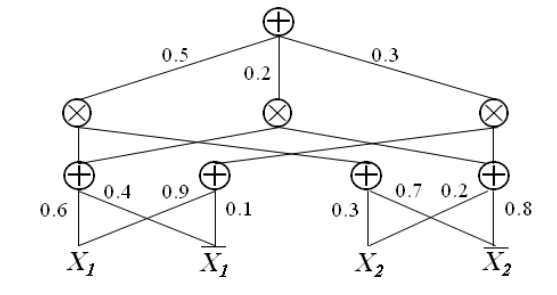
\includegraphics[scale=0.3]{spn_1.png}
                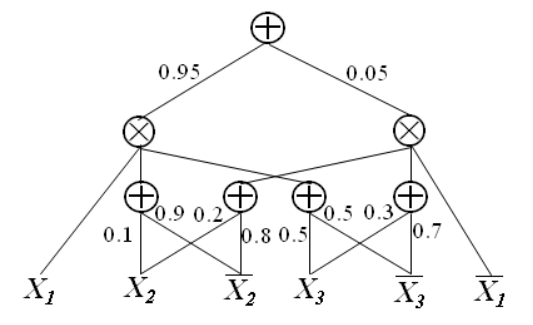
\includegraphics[scale=0.3]{spn_2.png}
                \caption{A esquerda uma SPN implementando uma naive Bayes mixture model. A direita uma SPN
    implementando uma junction tree. Fonte: Poon e Domingos\cite{poon-domingos}.}
              \end{figure}

              \begin{spn-def} Uma SPN $S$ é válida sse $S(e)=\Phi_S(e)$ para toda evidência $e$,
                onde $\Phi_S$ é a distribuição de probabilidade não-normalizada da SPN $S$.
              \end{spn-def} \\~\\

              \begin{spn-def} Uma SPN é \emph{completa} sse todos os filhos do mesmo nó soma tem
                mesmo escopo.
              \end{spn-def} \\~\\

              \begin{spn-def} Uma SPN é \emph{consistente} sse nenhuma variável aparece negada em
                um filho de um nó produto e não-negada em outro.
              \end{spn-def} \\~\\

              \begin{spn-thm} Uma SPN é válida se ela é completa e consistente.
              \end{spn-thm} \\~\\

              SPNs válidas são desejáveis pois uma SPN válida computa a probabilidade de evidência
              em tempo linear em seu tamanho, além de completude e consistência permitirem que a
              inferência da SPN seja garantidamente eficiente.
\vspace*{0.2cm}
            \end{block}
\vspace*{0.2cm}
            \begin{block}{Aprendizado}
                \justifying
                  Podemos gerar uma SPN por aprendizado criando uma SPN densa inicialmente e em
                  seguida aprendermos os pesos. Domingos e Poon\cite{poon-domingos} sugerem um
                  algoritmo que cria uma SPN inicial e em seguida aprende os pesos por Gradient
                  Descent ou Expectation-Maximization (EM) que é mostrada na seção Algoritmo de
                  Aprendizado. No entanto, há outros jeitos de se aprender uma SPN. \\~\\

                  Gens e Domingos\cite{gens-domingos} desenvolveram um método de aprendizado que
                  explora dependência e independência dos dados do conjunto de treino para melhorar
                  a flexibilidade e custo de aprendizado de uma SPN. O método proposto usa a
                  expressividade da estrutura de SPNs para alcançar resultados superiores aos
                  experimentos realizados anteriormente. \\~\\

                  Outros métodos de aprendizado incluem buscas gulosas\cite{greedy-search},
                  clustering de variáveis\cite{clustering} e o uso de Non-Parametric Bayesian
                  Sum-Product Networks\cite{non-parametric-bayesian}.
            \end{block}
          }
        \end{minipage}
      \end{beamercolorbox}
    \end{column}
    % ---------------------------------------------------------%
    % end the column

    % ---------------------------------------------------------%
    % Set up a column
    \begin{column}{.5\textwidth}
      \begin{beamercolorbox}[center,wd=\textwidth]{postercolumn}
        \begin{minipage}[T]{.95\textwidth} % tweaks the width, makes a new \textwidth
          \parbox[t][\columnheight]{\textwidth}{ % must be some better way to set the the height, width and textwidth simultaneously
            % Since all columns are the same length, it is all nice and tidy.  You have to get the height empirically
            % ---------------------------------------------------------%
            % fill each column with content

\vspace*{0.2cm}
            \begin{block}{Algoritmo de Aprendizado}

              \begin{algorithm}[H]
                \NoCaptionOfAlgo
                \KwIn{Conjunto $D$ de instâncias sobre variáveis $X$.}
                \KwOut{Uma SPN com estrutura e parâmetros construídos por aprendizado.}
                \tcc{Cria uma SPN inicial que seja válida.}
                $S \leftarrow$ GenerateDenseSPN($X$)\;
                InitializeWeights($S$)\;
                \Repeat{convergência}{
                  \ForAll{$d \in D$}{
                    \tcc{Atualiza pesos por Gradient Descent ou EM.}
                    UpdateWeights($S$, Inference($S$, $d$))\;
                  }
                }
                \tcc{Apara arestas com peso $w_{ij}=0$ e nós não-raíz sem pais.}
                $S \leftarrow$ PruneZeroWeights($S$)\;
                \KwRet{$S$}
              \end{algorithm}
\vspace*{0.2cm}
            \end{block}
\vspace*{0.2cm}
            \begin{block}{Experimentos}
            \justifying
              Os experimentos mostrados a seguir foram extraídos a partir da implementação do
              algoritmo mostrado na seção anterior e mostram os resultados do código
              \cite{website:poon-domingos-code} implementado por Domingos e Poon e citados em
              \cite{poon-domingos}.

              \begin{figure}[h]
                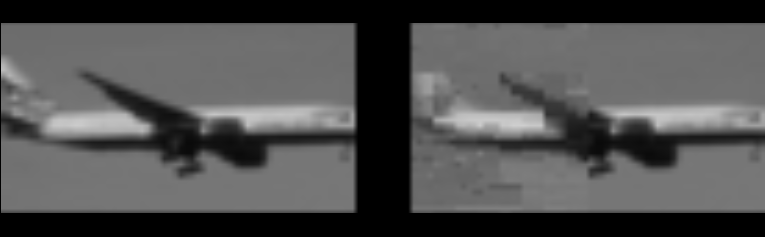
\includegraphics[scale=0.3]{completions/plane0.png}
                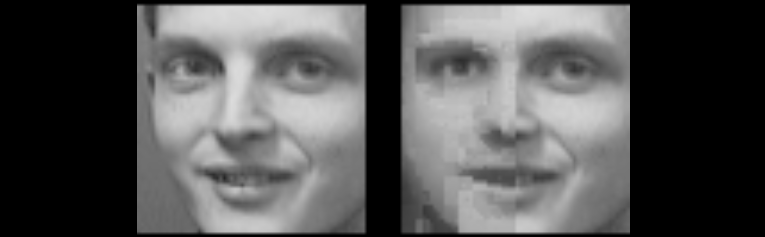
\includegraphics[scale=0.3]{completions/face0.png} \\
                
\includegraphics[scale=0.3]{completions/stop0.png}
                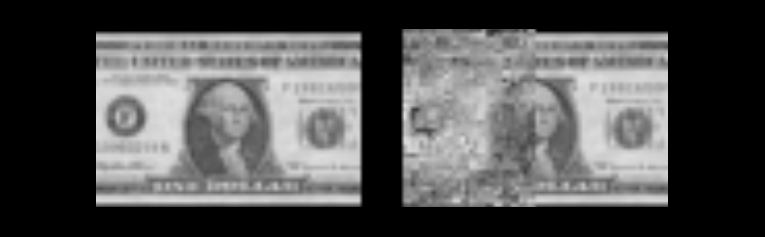
\includegraphics[scale=0.3]{completions/dollar0.png}
                \caption{A saída do algoritmo consiste na compleção do lado esquerdo das imagens
                  a partir de um conjunto de treino. Para cada par de imagens, a imagem da esquerda
                  é a original, enquanto que a direita tem a metade esquerda completada pela SPN
                  e a outra metade igual a da original como evidência.}
              \end{figure}

              \begin{table}[h]
                \begin{center}
                  \begin{tabular}{l | r | r | r}
                    Arquitetura & Rostos & Motos & Carros \\
                    \hline
                    SPN & 0.99 & 0.99 & 0.98 \\
                    CDBN & 0.95 & 0.81 & 0.87 \\
                  \end{tabular}
                \end{center}
                \caption{Comparação entre SPNs e CDBNs (Convolutional Deep Belief Networks) em
                  classificação (reconhecimento) de imagens.}
              \end{table}

              Pode-se ver que os resultados das SPNs são muito promissores e, dado que o algoritmo
              produzido por Domingos e Poon não toma muita vantagem da expressividade da estrutura
              local de SPNs, é fácil notar que ainda há muito espaço para melhorias.

\vspace*{0.2cm}
            \end{block}
\vspace*{0.2cm}
            \begin{block}{Trabalhos futuros}
              \justifying
                Pretende-se estudar a implementação do método de aprendizado proposto por Poon e
                Domingos\cite{poon-domingos} e explorar mais a fundo as propriedades de uma SPN,
                principalmente o uso de estrutura local para tornar o aprendizado mais rápido e
                preciso.\\~\\

                Em seguida planeja-se estudar outros tipos de aprendizado em SPNs, como o
                introduzido por Gens e Domingos\cite{gens-domingos}, buscas gulosas e clustering
                por Dennis e Ventura\cite{clustering, greedy-search} e Non-Parametric Bayesian
                Sum-Product Networks\cite{non-parametric-bayesian}.

            \end{block}
\vspace*{0.2cm}
            \begin{block}{Referências}
            \scriptsize
            \bibliographystyle{alpha}
            \bibliography{references}
\vspace*{0.2cm}
            \end{block}
            \vfill
          }
        \end{minipage}
      \end{beamercolorbox}
    \end{column}
    % ---------------------------------------------------------%
    % end the column


  \end{columns}
\end{frame}


\end{document}


%%%%%%%%%%%%%%%%%%%%%%%%%%%%%%%%%%%%%%%%%%%%%%%%%%%%%%%%%%%%%%%%%%%%%%%%%%%%%%%%%%%%%%%%%%%%%%%%%%%%
%%% Local Variables:
%%% mode: latex
%%% TeX-PDF-mode: t
%%% End:
